\documentclass[a4paper,10pt,report]{amsart}
    \usepackage{bm,amsmath,amssymb,framed,cases,euscript,cleveref,newtxtext,newtxmath}
    \usepackage{remreset}
    \usepackage[dvipdfmx]{graphicx}
    \makeatletter
        \renewcommand{\theequation}{% 式番号の付け方
        \thesection.\arabic{equation}}
        \@addtoreset{equation}{section}
    
        \renewcommand{\thetable}{% 表番号の付け方
        \thesection.\arabic{table}}
        \@addtoreset{table}{section}
    \makeatother
    %
    \theoremstyle{plain}
    %
    \theoremstyle{definition}
    \newtheorem{defn}{Def.}[section]
    \newtheorem{thm}{Thm.}[section]
    \newtheorem{lem}{Lem.}[section]
    \newtheorem{cor}{Cor.}[section]
    \newtheorem{prop}{Prop.}[section]
    \newtheorem{law}{Law.}
    \newtheorem{req}{Req.}[section]
    \crefname{req}{Requirement}{Requirements}
    %
    \theoremstyle{remark}
    \newtheorem{rem}{Rem}
    \newtheorem{prf}{Prf.}
%
    \let\normalref\ref
\renewcommand{\ref}{\cref}
    %
    %
    \title{Answer for 1B 2016}
    \author{Naoki Yano}
    \date{\today}
    %
\begin{document}
    \maketitle
    \begin{enumerate}
        \item 
        \begin{equation*}
            \frac{x^{3}-3}{x^{3}-x^{2}-x+1}=\frac{x^{3}-x^{2}-x+1+(x^{2}+x-4)}{x^{3}-x^{2}-x+1}
        \end{equation*}
        \begin{equation*}
            =1+\frac{x^{2}+x-4}{x^{3}-x^{2}-x+1}
        \end{equation*}
        ここで
        \begin{equation*}
            x^{3}-x^{2}-x+1={(x-1)}^{2}(x+1)
        \end{equation*}
        だから
        \begin{equation*}
            \frac{x^{2}+x-4}{x^{3}-x^{2}-x+1}=\frac{A}{{(x-1)}^{2}}+\frac{B}{x-1}+\frac{C}{x+1}
        \end{equation*}
        とおけて, 
        \begin{equation*}
            x^{2}+x-4=A(x+1)+B(x+1)(x-1)+C{(x-1)}^{2}
        \end{equation*}
        \begin{equation*}
            x^{2}+x-4=(B+C)x^{2}+(A-2B)x+A-B+C
        \end{equation*}
        係数を比較して,
        \begin{equation*}
            \begin{cases}
                B+C=1\\
                A-2B=1\\
                A-B-C=-4
            \end{cases}
        \end{equation*}
        これを拡大係数行列にして連立方程式を解くと, 
        \begin{equation*}
            \begin{bmatrix}
                0 & 1 & 1 & 1\\
                1 & -2 & 0 & 1\\
                1 & -1 & -1 & -4
            \end{bmatrix}
            \to \begin{bmatrix}
                1 & -1 & -1 & -4\\
                0 & 1 & 1 & 1\\
                0 & 0 & 1 & 3
            \end{bmatrix}
        \end{equation*}
        \begin{equation*}
            \therefore C=3,B=-2,A=-3
        \end{equation*}
        \begin{equation*}
            I=\int1dx+\int\left(\frac{-3}{{(x-1)}^{2}}+\frac{-2}{x-1}+\frac{1}{x+1}\right)dx
        \end{equation*}
        \begin{equation*}
            =x+\frac{3}{x-1}+\log\left|\frac{x+1}{{(x-1)}^{2}}\right|+\mathrm{const.}
        \end{equation*}
        \item
        \begin{equation*}
            \mathcal{D}:=\{(x,y)\mid0\leq y\leq 1,y^{3}\leq x\leq 2-y^{2}\}
        \end{equation*}
        これをグラフに書くと
        \begin{figure}[tbh]
            \centering
            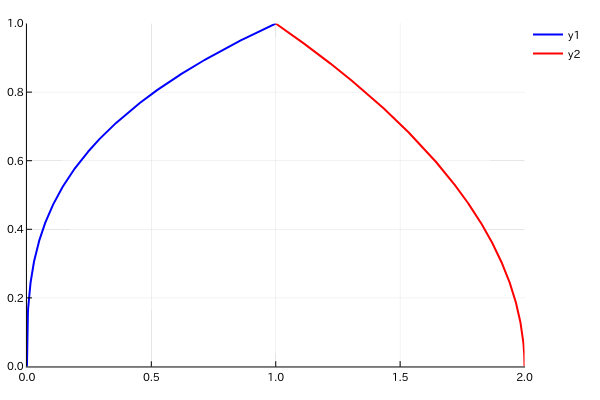
\includegraphics[height=7cm]{newplot.png}
            \caption{\(y_{1}:y=\sqrt[3]{x},y_{2}:y=\sqrt{2-x}\)のグラフ. }
        \end{figure}
        \begin{equation*}
            \mathcal{D}'=\left \{(x,y)\middle|0\leq x\leq 2,
            \begin{cases}
                0\leq y\leq \sqrt[3]{x}&(0\leq x\leq 1) \\
                0\leq y\leq \sqrt{2-x}&(1\leq x\leq 2)
            \end{cases}
            \right \}
        \end{equation*}
        從って定積分は
        \begin{equation*}
            I=\int_{0}^{1}\left(\int_{0}^{\sqrt[3]{x}}\frac{y^{2}}{x\sqrt{2-x}}dy\right)dx+\int_{1}^{2}\left(\int_{0}^{\sqrt{2-x}}\frac{y^{2}}{x\sqrt{2-x}}dy\right)dx
        \end{equation*}
        \begin{equation*}
            =\int_{0}^{1}\frac{1}{3\sqrt{2-x}}dx+\int_{1}^{2}\frac{2-x}{3x}dx={\left[-\frac{2}{3}\sqrt{2-x}\right]}_{0}^{1}+{\left[\frac{2}{3}\log{}x\right]}_{1}^{2}-{\left[\frac{1}{3}x\right]}_{1}^{2}
        \end{equation*}
        \begin{equation*}
            =\frac{2}{3}(\sqrt{2}+\log{2})-1
        \end{equation*}
        \item 
        \begin{equation*}
            \mathcal{D}:=\{(x,y)\mid{}x^{2}+y^{2}\leq4\}
        \end{equation*}
        \begin{equation*}
            f_{x}=\frac{x}{2\sqrt{x^{2}+y^{2}}}\exp{\frac{\sqrt{x^{2}+y^{2}}}{2}}-\frac{x}{2\sqrt{x^{2}+y^{2}}}\exp-{\frac{\sqrt{x^{2}+y^{2}}}{2}}
        \end{equation*}
        \begin{equation*}
            f_{y}=\frac{y}{2\sqrt{x^{2}+y^{2}}}\exp{\frac{\sqrt{x^{2}+y^{2}}}{2}}-\frac{y}{2\sqrt{x^{2}+y^{2}}}\exp-{\frac{\sqrt{x^{2}+y^{2}}}{2}}.
        \end{equation*}
        曲面積は
        \begin{equation*}
            S=\iint_{\mathcal{D}}\sqrt{1+f_{x}^{2}+f_{y}^{2}}dxdy=\iint_{\mathcal{D}}\sqrt{1+\frac{1}{4}{\left(\exp{\frac{\sqrt{x^{2}+y^{2}}}{2}}-\exp-{\frac{\sqrt{x^{2}+y^{2}}}{2}}\right)}^{2}}dxdy.
        \end{equation*}
        ここで
        \begin{equation*}
            x=r\cos{x},y=\sin{x}
        \end{equation*}
        と変数変換すると, 
        \begin{equation*}
            S=\int_{0}^{2\pi}d\theta\int_{0}^{2}rdr\sqrt{\frac{1}{2}+\frac{1}{4}\left(\exp{r}+\exp{(-r)}\right)}
        \end{equation*}
        \begin{equation*}
            =\int_{0}^{2\pi}d\theta\int_{0}^{2}rdr\frac{1}{2}\sqrt{\left(\exp{r}+2+\exp{(-r)}\right)}=\int_{0}^{2\pi}d\theta\int_{0}^{2}rdr\frac{1}{2}\left(\exp{\frac{r}{2}}+\exp{\frac{-r}{2}}\right)
        \end{equation*}
        \begin{equation*}
            =\int_{0}^{2\pi}d\theta\int_{0}^{1}u\left(\exp{u}+\exp{-u}\right)du=2\pi {[u\exp{u}-\exp{u}-u\exp{-u}-\exp{-u}]}_{0}^{1}
        \end{equation*}
        \begin{equation*}
            =2\pi(1-2e^{-1})
        \end{equation*}
        \item 
        \begin{enumerate}
            \item 
            \begin{equation*}
                \varphi(x,y,z)=\exp{(-x^{2}-y^{2})}-z
            \end{equation*}
            とおくと, 問題の曲面は\(\varphi=0\)で表される曲面である. この曲面の法線ベクトルは
            \begin{equation*}
                \nabla \varphi=\begin{bmatrix}
                    -2x\exp{(-x^{2}-y^{2})}\\
                    -2y\exp{(-x^{2}-y^{2})}\\
                    -1
                \end{bmatrix}
            \end{equation*}
            從って求める単位法線ベクトルは
            \begin{equation*}
                \bm{n}=\frac{1}{\sqrt{4(x^{2}+y^{2})\exp{(-2(x^{2}+y^{2}))}+1}}\begin{bmatrix}
                    2x\exp{(-x^{2}-y^{2})}\\
                    2y\exp{(-x^{2}-y^{2})}\\
                    1
                \end{bmatrix}
            \end{equation*}
            \item 
            \begin{equation*}
                \bm{f}=\begin{bmatrix}
                    x\\
                    y\\
                    z
                \end{bmatrix}
            \end{equation*}
            だから
            \begin{equation*}
                \bm{f}\cdot\bm{n}=\frac{\{2(x^{2}+y^{2})+1\}\exp{(-(x^{2}+y^{2}))}}{\sqrt{4(x^{2}+y^{2})\exp{(-2(x^{2}+y^{2}))}+1}}
            \end{equation*}
            また\(dS\)は
            \begin{equation*}
                dS=\sqrt{1+\varphi_{x}^{2}+\varphi_{y}^{2}}dxdy=\sqrt{4(x^{2}+y^{2})\exp{-2(x^{2}-y^{2})}+1}
            \end{equation*}
            從って求める面積分は
            \begin{equation*}
            S=\iint_{\mathcal{D}}\bm{f}\cdot\bm{n}dS=\iint_{\mathcal{D}}\{2(x^{2}+y^{2})+1\}\exp(-x^{2}-y^{2})
            \end{equation*}
            ここで
            \begin{equation*}
                x=r\cos{x},y=\sin{x}
            \end{equation*}
            と変数変換すると, 
            \begin{equation*}
                S=\int_{0}^{\frac{\pi}{2}}d\theta\int_{0}^{\infty}rdr(2r^{2}+1)\exp{(-r^{2})}=\int_{0}^{\frac{\pi}{2}}d\theta\int_{0}^{\infty}(2r^{2}+1)r\exp(-r^{2})dr
            \end{equation*}
            \begin{equation*}
                =\int_{0}^{\frac{\pi}{2}}d\theta\left\{{\left[-\frac{1}{2}(2r^{2}+1)\exp(-r^{2})\right]}_{0}^{\infty}+\int_{0}^{\infty}\frac{1}{2}(4r)\exp(-r^{2})dr\right\}
            \end{equation*}
            \begin{equation*}
                =\int_{0}^{\frac{\pi}{2}}d\theta\left(\frac{1}{2}+{[-\exp(-r^{2})]}_{0}^{\infty}\right)=\frac{3}{2}\frac{\pi}{2}
            \end{equation*}
            \begin{equation*}
                =\frac{3}{4}\pi
            \end{equation*}
        \end{enumerate}
        \item Greenの定理から
        \begin{equation*}
            I=\int_{\Gamma}(\sin{x}+e^{x})\sin{y}dx+(\cos{x}+e^{x})\cos{y}dy=\iint_{S}\left \{-\frac{\partial}{\partial y}(\sin{x}+e^{x})\sin{y}+\frac{\partial}{\partial x}(\cos{x}+e^{x})\cos{y}\right \}dxdy
        \end{equation*}
        \begin{equation*}
            =\iint_{S}\{-(\sin{x}+e^{x})\cos{y}+(-\sin{x}+e^{x})\cos{y}\}dxdy=\iint_{S}(-2\sin{x}\cos{y})dxdy. 
        \end{equation*}
        ここで
        \begin{equation*}
            u=\frac{1}{\sqrt{2}}(x+y),v=\frac{1}{\sqrt{2}}(-x+y)
        \end{equation*}
        と変数変換すると, 
        \begin{equation*}
            S=\left\{(u,v)\middle| 0\leq u\leq\frac{\sqrt{2}\pi}{4},0\leq v\leq \frac{\sqrt{2}\pi}{6}\right\}
        \end{equation*}
        \begin{equation*}
            x=\frac{1}{\sqrt{2}}(u-v),y=\frac{1}{\sqrt{2}}(u+v).
        \end{equation*}
        \begin{equation*}
            J(u,v)=\left|\begin{array}{cc}
                \frac{1}{\sqrt{2}} & -\frac{1}{\sqrt{2}}\\
                \frac{1}{\sqrt{2}} & \frac{1}{\sqrt{2}}
            \end{array}\right|=1
        \end{equation*}
        \begin{equation*}
            \therefore I=\int_{0}^{\frac{\sqrt{2}\pi}{4}}du\int_{0}^{\frac{\sqrt{2}\pi}{6}}dv-2\sin{\frac{1}{\sqrt{2}}(u-v)}\cos{\frac{1}{\sqrt{2}}(u+v)}
        \end{equation*}
        積和の公式から
        \begin{equation*}
            \sin{\frac{1}{\sqrt{2}}(u-v)}\cos{\frac{1}{\sqrt{2}}(u+v)}=\frac{1}{2}(\sin{\sqrt{2}u}-\sin{\sqrt{2}v})
        \end{equation*}
        だから,
        \begin{equation*}
            I=\int_{0}^{\frac{\sqrt{2}\pi}{4}}du\int_{0}^{\frac{\sqrt{2}\pi}{6}}dv(-\sin{\sqrt{2}u}+\sin{\sqrt{2}v})
        \end{equation*}
        \begin{equation*}
            =\int_{0}^{\frac{\sqrt{2}\pi}{4}}{\left[-v\sin{\sqrt{2}u}+\frac{1}{\sqrt{2}}\cos{\sqrt{2}v}\right]}_{0}^{\frac{\sqrt{2}\pi}{6}}du=\int_{0}^{\frac{\sqrt{2}\pi}{4}}{\left[-\frac{\sqrt{2}\pi}{6}\sin{\sqrt{2}u}+\frac{1}{2\sqrt{2}}-\frac{1}{\sqrt{2}}\right]}du
        \end{equation*}
        \begin{equation*}
            =\left[\frac{\pi}{6}\cos{\sqrt{2}u}-\frac{u}{\sqrt{2}}\right]_{0}^{\frac{\sqrt{2}\pi}{4}}=0-\frac{\pi}{4}-\frac{\pi}{6}
        \end{equation*}
        \begin{equation*}
            =-\frac{\pi}{12}.
        \end{equation*}
    \end{enumerate}
    %
\end{document}